%% TMLR submission (double-blind).
%% Requires tmlr.sty and tmlr.bst from the official TMLR template next to main.tex.
%% Build: pdflatex main && bibtex main && pdflatex main && pdflatex main
%%
%% Options: \usepackage{tmlr}            submission (authors hidden, anonymous)
%%          \usepackage[preprint]{tmlr}  de-anonymized preprint
%%          \usepackage[accepted]{tmlr}  camera-ready (fill \month, \year, \openreview)
\documentclass{article}
\usepackage{tmlr}

\usepackage{amsmath,amssymb}
\usepackage{booktabs}
\usepackage{array}
\usepackage{graphicx}
\usepackage{tikz}
\usetikzlibrary{positioning,arrows.meta,calc}
\usepackage{url}
\usepackage{placeins}
\usepackage{hyperref}
\hypersetup{pdfauthor={},pdftitle={Missing-Modality Audit}}
\raggedbottom

\newcommand{\pq}{PathQ-Former}
\newcommand{\cindex}{C-index}
\newcommand{\pmv}[2]{#1\,$\pm$\,#2}
\newcolumntype{R}[1]{>{\raggedright\arraybackslash}p{#1}}

\title{Do Histology--Transcriptomics Survival Models Use Both Inputs? A Missing-Modality Audit and a One-Checkpoint Training Recipe}

%% camera-ready: author block (hidden under \usepackage{tmlr} without options)
\author{\name Anonymous Author \email anonymous@example.org \\
      \addr Anonymous Institution}

\def\month{MM}  % camera-ready only
\def\year{YYYY} % camera-ready only
\def\openreview{\url{https://openreview.net/forum?id=XXXX}} % camera-ready only
\begin{document}

\maketitle

\begin{abstract}
Survival models that fuse whole-slide images (WSIs) with transcriptomics are evaluated on patients with both inputs, leaving two questions open: does the fused model use both, and what happens when one is missing? We audit this on five TCGA cohorts under one equal-budget, three-seed protocol by re-evaluating checkpoints with an input removed or permuted across patients. The official SurvPath implementation ranks patients the same way when its RNA input is permuted ($\Delta$\cindex{} $+0.001$) but loses 0.068 when the slide is permuted and falls to 0.47--0.52 without it. A query-bottleneck fusion model trained with null codes and modality dropout is equally blind to RNA removal but loses only 0.030 without the slide; auxiliary unimodal heads make the fused prediction respond to RNA ($-0.023$ under permutation), and one checkpoint keeps a \cindex{} of 0.54--0.62 with either input removed and moves at most 0.025 when half the patients lack a modality. With both inputs it does not detectably beat an RNA-only MLP or a late-fusion ensemble, and its $+0.036$ margin over the untuned SurvPath is significant under the Wilcoxon test but not the $t$-test. Replayed on stored histories, validation-loss early stopping would have cost it up to 0.09 \cindex{} and SurvPath nothing.
\end{abstract}

\section{Introduction}
\label{sec:intro}

Prognostic models in oncology draw on two kinds of evidence: histology records the phenotype of a tumour, and transcriptomics records the molecular state behind it. Pathology foundation models~\citep{chen2024uni,xu2024gigapath,vorontsov2024virchow} turn a gigapixel whole-slide image (WSI) into a few thousand frozen patch embeddings, and co-attention between patch tokens and gene or pathway tokens~\citep{chen2021mcat,jaume2024survpath} relates the two sets, so models that fuse WSIs with bulk gene expression report higher concordance than either modality alone on most cohorts of The Cancer Genome Atlas (TCGA)~\citep{chen2022pancancer,jaume2024survpath,song2024mmp}.\footnote{A large language model assisted with drafting and editing the text and \LaTeX{} source and with writing analysis and plotting code, under the authors' direction. The authors designed the study, ran the experiments, checked every reported number against the archived results, and are responsible for all content.}

Such models are evaluated on patients who have both inputs, which leaves two questions open. Does the fused model use both inputs? A concordance index (\cindex{}) measures how well predicted risks rank patients; it cannot show which input produced the ranking. And what happens when one input is missing, the normal state of a hospital cohort, where sequencing is not ordered for every patient and not every slide is digitised? We answer both with an input-use audit: every trained checkpoint is re-evaluated with one input removed, with one input permuted across patients, and with a random fraction of patients lacking a modality, and its fused risk scores are correlated with the risks of its own single-input evaluations. Applied under one protocol to the official SurvPath implementation~\citep{jaume2024survpath}, the audit finds that SurvPath's ranking does not respond to its RNA input ($\Delta$\cindex{} $+0.001$ under permutation across patients) and collapses when the slide is permuted ($\Delta$\cindex{} $-0.068$) or removed (\cindex{} 0.47--0.52).

The second part of the paper asks which training choices change this. We train one query-bottleneck fusion model, \pq{}, in two variants that differ only in training. With learned null codes and modality dropout alone, the model is as blind to RNA as SurvPath ($\Delta$\cindex{} $0.000$ with RNA removed) but no longer collapses without the slide ($-0.030$ instead of SurvPath's $-0.073$). Adding auxiliary unimodal survival heads makes the fused prediction respond to RNA ($-0.023$ under permutation); the resulting checkpoint keeps a \cindex{} of 0.54--0.62 with either input removed and changes by at most 0.025 when half of the patients lack a modality. With both inputs present, neither variant is detectably better than an RNA-only multilayer perceptron (MLP) or a late-fusion ensemble of two unimodal models, so the recipe buys coverage of incomplete patients, not accuracy. Our contributions are:
\begin{itemize}
\item An input-use audit (removal, permutation across patients, risk-score correlation; 3 seeds $\times$ 5 folds $\times$ 5 cohorts) applied to a published co-attention model under an equal-budget protocol (Section~\ref{sec:audit}). SurvPath's ranking does not respond to its RNA input; a high fused \cindex{} does not show that both modalities are used.
\item Evidence on where missing-modality robustness comes from, from matched variants of one fusion model (Sections~\ref{sec:missing}--\ref{sec:where}): null codes and modality dropout remove the collapse without the slide ($-0.030$ with the null code against $-0.069$ with mean imputation on the same checkpoints, one seed, and $-0.073$ for SurvPath); auxiliary unimodal heads are what makes the fused output respond to RNA; the single checkpoint matches an RNA-only MLP and a late-fusion ensemble with both inputs and works with either input absent.
\item Protocol evidence that this literature rarely reports (Sections~\ref{sec:accuracy} and~\ref{sec:selection}): equal-budget accuracy with seed-aware statistics (seed-averaged 25-fold paired tests with bootstrap confidence intervals and Holm correction), and a post-hoc replay of checkpoint selection on event-poor folds from the stored training histories.
\end{itemize}

\paragraph{Scope of claims} SurvPath was run with its published hyper-parameters and was not re-tuned under our protocol. \pq{}'s hyper-parameters were developed on the bladder cohort (BLCA) under a 10-epoch budget, and the auxiliary-head variant and its loss weight were adopted after the 20-epoch results on all five cohorts had been seen, so both variants are reported as co-primary and no accuracy superiority over SurvPath is claimed. The training recipe has not been applied to SurvPath. All results are on TCGA with frozen UNI2-h features, simulated missingness is random and therefore uninformative, and no clinical covariates are modelled.

\section{Related Work}
\label{sec:related}

\paragraph{Fusion of WSIs and genomics} WSIs are processed as bags of patches under multiple-instance learning: attention-based MIL (ABMIL)~\citep{ilse2018abmil}, clustering-constrained attention MIL (CLAM)~\citep{lu2021clam} and TransMIL~\citep{shao2021transmil} pool patch features from self-supervised~\citep{wang2022ctranspath} or foundation-model encoders trained on $10^8$ patches or more~\citep{chen2024uni,xu2024gigapath,vorontsov2024virchow}. Early fusion work concatenated convolutional neural network (CNN) and genomic features~\citep{mobadersany2018predicting} or combined unimodal representations with Kronecker products and gating~\citep{chen2022pathomic}; a pan-cancer study found that fusion improved concordance in 12 of 14 cancer types~\citep{chen2022pancancer}. MCAT~\citep{chen2021mcat} introduced co-attention from functional gene groups to patches; SurvPath~\citep{jaume2024survpath} replaced the groups with Reactome and Hallmark pathway tokens and modelled dense pathway--patch interactions in one Transformer; MOTCat~\citep{xu2023motcat}, CMTA~\citep{zhou2023cmta}, PIBD~\citep{zhang2024pibd} and MMP~\citep{song2024mmp}, which reports gains over SurvPath, vary the interaction, and continually evolved multimodal foundation models extend the setting~\citep{peng2025continual}. Two-bank learned-query fusion over patches and pathways already exists in APL~\citep{liu2025apl}; the query bottleneck used here is not claimed as new.

\paragraph{Missing modalities in multimodal survival} Modality dropout was introduced for gesture recognition~\citep{neverova2016moddrop} and applied to pan-cancer prognosis by \citet{cheerla2019deep} and MultiSurv~\citep{valesilva2021long}. \citet{ma2022robust} showed that multimodal Transformers are not robust to missing inputs by default; SMIL~\citep{ma2021smil}, ShaSpec~\citep{wang2023shaspec} and missing-aware prompts~\citep{lee2023prompt} address it with meta-learning, shared--specific features or prompt tokens. For WSIs and genomics, G-HANet~\citep{wang2024ghanet} distils genomic knowledge into a histology-only model, and recent work binds incomplete modalities~\citep{qu2024binding}, distils prompts~\citep{xu2025dispro}, learns conditional latent variables~\citep{zhou2025ldcvae}, uses prototype-guided cross-modal knowledge~\citep{liu2025prosurv}, memory-augmented hypergraphs~\citep{qu2025m2surv} or prototype-driven pretraining~\citep{yu2026prime}. None of these audits whether a published co-attention model uses its genomic input, nor tests under equal budgets whether unimodal auxiliary supervision changes that; this is the gap we address.

\paragraph{Learned queries} A set of learned vectors that cross-attend to a large input and return a fixed-size summary appears as inducing points~\citep{lee2019set}, object queries~\citep{carion2020detr}, the Perceiver latent array~\citep{jaegle2021perceiver}, the Perceiver Resampler~\citep{alayrac2022flamingo}, the Q-Former~\citep{li2023blip2} and the prototype banks of APL~\citep{liu2025apl}. The property used here is that the output has a fixed shape, so an absent input can be replaced by a learned tensor of the same shape.

\paragraph{Modality imbalance} Gradient Blending~\citep{wang2020gradientblending} and OGM-GE~\citep{peng2022ogmge} showed that joint training lets one modality dominate and counteract it with per-modality supervision or gradient modulation. The auxiliary unimodal heads used here are unimodal supervision in that tradition, not a new idea; our contribution is to measure what they change in a survival-fusion model under an audit.

\section{Experimental Setup}
\label{sec:setup}

\subsection{Data and cohorts}
Five TCGA cohorts are used (Table~\ref{tab:cohorts}): bladder urothelial carcinoma (BLCA), breast invasive carcinoma (BRCA), colorectal adenocarcinoma (COADREAD), head and neck squamous cell carcinoma (HNSC) and stomach adenocarcinoma (STAD). Patch embeddings are the released 1,536-d UNI2-h features~\citep{chen2024uni,uni2h,uni2hfeatures}, used as released. The RNA-seq matrices (4,999 genes), clinical metadata and five-fold patient-level splits are those released with SurvPath~\citep{jaume2024survpath}. The primary endpoint is disease-specific survival (DSS) from the TCGA Clinical Data Resource~\citep{liu2018integrated}; overall survival (OS) is secondary. The split is fixed per cohort, so fold $k$ holds the same validation patients for every method and seed, and the number of events in a validation fold ranges from 5 to 45 (median 16).

\begin{table}[t]
\caption{Cohorts as realised by the DSS splits (every method and seed uses the same five folds). Patients and events per validation fold are the minimum--maximum over the five folds. $^\dagger$Development cohort for \pq{}'s hyper-parameters.}
\label{tab:cohorts}
\centering
\small
\begin{tabular}{@{}llrrrr@{}}
\toprule
Cohort & Site & Patients & DSS events & Patients per fold & Events per fold \\
\midrule
BLCA$^\dagger$ & bladder & 359 & 113 & 70--75 & 16--25 \\
BRCA & breast & 868 & 60 & 166--182 & 7--20 \\
COADREAD & colon and rectum & 296 & 37 & 45--71 & 5--13 \\
HNSC & head and neck & 392 & 117 & 56--126 & 13--45 \\
STAD & stomach & 318 & 84 & 42--101 & 9--33 \\
\bottomrule
\end{tabular}
\end{table}

\subsection{Protocol}
\label{sec:protocol}
Table~\ref{tab:protocol} states the protocol, which is applied without change to every method. Every method trains for a fixed budget of 20 epochs and reports the final checkpoint, the convention of MCAT and SurvPath; no checkpoint is selected on the validation fold, which is also the reported fold. The budget was set after inspecting pooled validation curves under a 10-epoch budget (Appendix~\ref{app:training}), so 10-epoch results are reported as well. Appendix~\ref{app:pitfalls} lists evaluation pitfalls of survival MIL pipelines that the protocol avoids.

\begin{table}[t]
\caption{Evaluation protocol, identical for all methods.}
\label{tab:protocol}
\centering
\small
\begin{tabular}{@{}p{0.2\linewidth}p{0.76\linewidth}@{}}
\toprule
Aspect & Choice \\
\midrule
Unit of analysis & patient; all slides of a patient concatenated \\
Splits & SurvPath's five-fold patient-level cross-validation splits; the validation fold is the reported fold \\
Endpoint & disease-specific survival; overall survival as a secondary endpoint \\
Time bins & quartiles of uncensored training patients, outer edges $\pm\infty$, reused for validation \\
Primary metric & Harrell's \cindex{} on continuous time~\citep{harrell1982evaluating,polsterl2020scikit} \\
Secondary metrics & Uno's inverse-probability-of-censoring-weighted (IPCW) \cindex{}~\citep{uno2011c} truncated at the 75th percentile of training event times; integrated Brier score~\citep{graf1999assessment} on the interior quartile grid; log-rank test at the median risk split (Appendices~\ref{app:tables} and~\ref{app:km}) \\
Training budget & 20 epochs, final checkpoint, all methods \\
Seeds & three (0, 1, 2); the fold index is added to the seed \\
Statistics & one value per (cohort, fold) = mean over seeds; paired $t$ and Wilcoxon signed-rank tests over the 25 pooled folds with a 95\% percentile-bootstrap CI of the mean difference (10,000 resamples of folds) as the primary test; per-cohort tests ($n = 5$) are Holm-adjusted over the five cohorts and exploratory \\
Audit & the same checkpoint evaluated with each input removed or permuted across patients, with 10--50\% of patients missing one modality at random (five draws), and Spearman correlation between its fused and single-input risks \\
\bottomrule
\end{tabular}
\end{table}

\paragraph{Statistics} The three seeds of a fold share its validation patients, so (fold, seed) pairs are not independent replicates~\citep{nadeau2003inference}. The unit of analysis is therefore the (cohort, fold): the \cindex{} of each method is averaged over the seeds available for both methods, the paired difference is formed on each of the 25 folds, and a paired $t$-test, a two-sided exact Wilcoxon signed-rank test and a 95\% percentile-bootstrap confidence interval (CI) of the mean difference are computed over the folds. Per-cohort tests have five folds each; their $p$-values are Holm-adjusted over the five cohorts and are exploratory. ``Mean $\pm$ sd'' in a table is the mean and standard deviation over seeds of the five-fold mean unless the caption says otherwise.

\subsection{Methods}
\label{sec:methods}
Table~\ref{tab:methods} lists the methods and the seeds run for each. SurvPath, ABMIL, SNN and the RNA MLP use the hyper-parameters of the SurvPath repository; none was tuned under this protocol.

\begin{table}[t]
\caption{Methods and runs. ``Seeds'' is the number of seeds under the 20-epoch DSS protocol; one BRCA run of each single-modality \pq{} is missing at seed 2. Parameter counts include the pathway MLPs.}
\label{tab:methods}
\centering
\small
\setlength{\tabcolsep}{4pt}
\begin{tabular}{@{}R{0.26\linewidth}R{0.105\linewidth}R{0.29\linewidth}R{0.125\linewidth}R{0.15\linewidth}@{}}
\toprule
Method & Inputs & Training & Seeds & Also run under \\
\midrule
SurvPath (official)~\citep{jaume2024survpath} & WSI+RNA & published hyper-parameters; 21.2\,M params & 3 & OS (1); 10 epochs (3) \\
ABMIL~\citep{ilse2018abmil} & WSI & repository defaults & 3 & -- \\
SNN (self-normalizing network)~\citep{klambauer2017self} & RNA & repository defaults & 3 & -- \\
RNA MLP & RNA & two layers, repository defaults & 3 & -- \\
Slide-only \pq{} & WSI & trained with RNA absent & 3 (BRCA 2) & -- \\
RNA-only \pq{} & RNA & trained with slide absent & 3 (BRCA 2) & -- \\
Late fusion & WSI+RNA & mean of the $z$-scored risks of the slide-only and RNA-only \pq{}s (same seed) & 2 & -- \\
\pq{} w/o aux heads & WSI+RNA & null codes, modality dropout; 16.9\,M params & 3 & 10 epochs (3) \\
\pq{} & WSI+RNA & as above plus auxiliary heads, $\lambda = 0.5$ & 3 & OS (1) \\
\bottomrule
\end{tabular}
\end{table}

\begin{figure}[t]
\centering
% PathQ-Former overview: (a) training, (b) inference.
% Standalone tikzpicture; \input it inside a figure environment.
% Needs tikz with libraries positioning, arrows.meta, calc.
% Colours: histology = blue, transcriptomics = orange, shared parts = neutral gray.
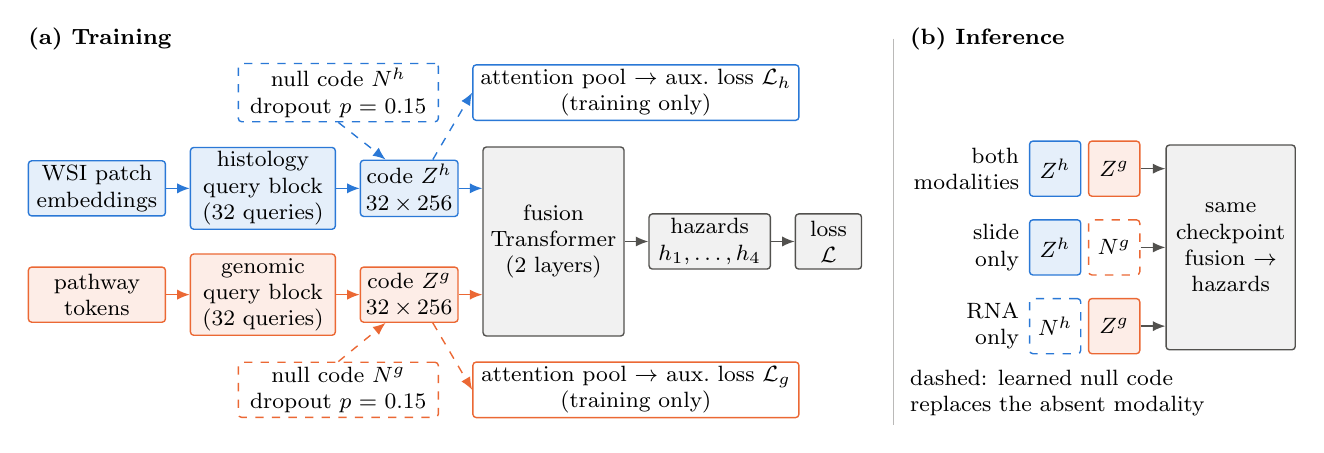
\begin{tikzpicture}[x=1mm, y=1mm, font=\footnotesize, line width=0.5pt,
  >={Latex[length=1.6mm, width=1.3mm]},
  box/.style={draw, rounded corners=1.2pt, align=center, inner xsep=2pt, inner ysep=1.5pt, minimum height=7mm},
  hbox/.style={box, draw=hist, fill=hist!12},
  gbox/.style={box, draw=gen, fill=gen!12},
  nbox/.style={box, draw=neut, fill=neut!8},
  hnull/.style={box, draw=hist, dashed, fill=white},
  gnull/.style={box, draw=gen, dashed, fill=white},
  haux/.style={box, draw=hist, fill=white},
  gaux/.style={box, draw=gen, fill=white},
  chip/.style={box, minimum width=6.5mm, minimum height=5.5mm, inner sep=1pt},
  harr/.style={->, hist},
  garr/.style={->, gen},
  narr/.style={->, neut},
  hdash/.style={->, hist, dashed},
  gdash/.style={->, gen, dashed},
  plab/.style={font=\footnotesize\bfseries, anchor=west, inner sep=0pt},
]
\definecolor{hist}{HTML}{2A78D6}
\definecolor{gen}{HTML}{EB6834}
\definecolor{neut}{HTML}{52514E}

% ---------------- (a) Training ----------------
\node[plab] at (0,32.5) {(a) Training};
\node[hbox, text width=16mm, anchor=west] (wsi) at (0,13.5) {WSI patch\\embeddings};
\node[gbox, text width=16mm, anchor=west] (rna) at (0,0)    {pathway\\tokens};
\node[hbox, text width=17mm, right=3mm of wsi] (qh) {histology\\query block\\(32 queries)};
\node[gbox, text width=17mm, right=3mm of rna] (qg) {genomic\\query block\\(32 queries)};
\node[hbox, text width=11mm, right=3mm of qh] (zh) {code $Z^h$\\$32 \times 256$};
\node[gbox, text width=11mm, right=3mm of qg] (zg) {code $Z^g$\\$32 \times 256$};
\coordinate (zmid) at ($(zh.east)!0.5!(zg.east)$);
\node[nbox, text width=16.5mm, minimum height=24mm, right=3mm of zmid] (fus) {fusion\\Transformer\\(2 layers)};
\node[nbox, text width=14mm, right=3mm of fus] (haz) {hazards\\$h_1,\dots,h_4$};
\node[nbox, text width=7mm,  right=3mm of haz] (loss) {loss\\$\mathcal{L}$};
% null codes (modality dropout) and auxiliary heads, above/below the code row
\node[hnull, text width=24mm] (nh) at ($(zh.north)+(-9mm,8.5mm)$) {null code $N^h$\\dropout $p = 0.15$};
\node[gnull, text width=24mm] (ng) at ($(zg.south)+(-9mm,-8.5mm)$) {null code $N^g$\\dropout $p = 0.15$};
\node[haux, text width=40mm, anchor=west] (ah) at ($(zh.north)+(8mm,8.5mm)$)  {attention pool $\to$ aux.\ loss $\mathcal{L}_h$\\(training only)};
\node[gaux, text width=40mm, anchor=west] (ag) at ($(zg.south)+(8mm,-8.5mm)$) {attention pool $\to$ aux.\ loss $\mathcal{L}_g$\\(training only)};
% main flow
\draw[harr] (wsi) -- (qh);
\draw[harr] (qh) -- (zh);
\draw[harr] (zh.east) -- (zh.east -| fus.west);
\draw[garr] (rna) -- (qg);
\draw[garr] (qg) -- (zg);
\draw[garr] (zg.east) -- (zg.east -| fus.west);
\draw[narr] (fus) -- (haz);
\draw[narr] (haz) -- (loss);
% modality dropout: the null code replaces the code
\draw[hdash] (nh.south) -- ([xshift=-3mm]zh.north);
\draw[gdash] (ng.north) -- ([xshift=-3mm]zg.south);
% auxiliary unimodal heads (training only)
\draw[hdash] ([xshift=3mm]zh.north) -- (ah.west);
\draw[gdash] ([xshift=3mm]zg.south) -- (ag.west);

% ---------------- (b) Inference ----------------
\coordinate (b0) at (loss.east |- 0,0);
\draw[neut!40] ($(b0)+(4,32.5)$) -- ($(b0)+(4,-16.5)$);
\node[plab] at ($(b0)+(6,32.5)$) {(b) Inference};
\node[anchor=east, align=right, inner sep=0pt] at ($(b0)+(20,16)$) {both\\modalities};
\node[anchor=east, align=right, inner sep=0pt] at ($(b0)+(20,6)$)  {slide\\only};
\node[anchor=east, align=right, inner sep=0pt] at ($(b0)+(20,-4)$) {RNA\\only};
\node[chip, hbox]  (c1h) at ($(b0)+(24.5,16)$) {$Z^h$};
\node[chip, gbox]  (c1g) at ($(b0)+(32,16)$)   {$Z^g$};
\node[chip, hbox]  (c2h) at ($(b0)+(24.5,6)$)  {$Z^h$};
\node[chip, gnull] (c2g) at ($(b0)+(32,6)$)    {$N^g$};
\node[chip, hnull] (c3h) at ($(b0)+(24.5,-4)$) {$N^h$};
\node[chip, gbox]  (c3g) at ($(b0)+(32,-4)$)   {$Z^g$};
\node[nbox, text width=15mm, minimum height=26mm, anchor=west] (ckpt) at ($(b0)+(38.5,6)$) {same\\checkpoint\\fusion $\to$\\hazards};
\draw[narr] (c1g.east) -- (c1g.east -| ckpt.west);
\draw[narr] (c2g.east) -- (c2g.east -| ckpt.west);
\draw[narr] (c3g.east) -- (c3g.east -| ckpt.west);
\node[anchor=north west, inner sep=0pt, align=left] at ($(b0)+(6,-9.5)$) {dashed: learned null code\\replaces the absent modality};
\end{tikzpicture}

\caption{\pq{} is trained for missingness and served from one checkpoint. (a) Training. The WSI patch embeddings and the pathway tokens are each read by a block of 32 learned queries, giving codes $Z^h, Z^g \in \mathbb{R}^{32 \times 256}$ that a two-layer fusion Transformer maps to four discrete-time hazards and the survival loss $\mathcal{L}$. With probability $p = 0.15$ per sample, modality dropout replaces a present code by its learned null code $N^h$ or $N^g$ (dashed), and auxiliary survival losses $\mathcal{L}_h$ and $\mathcal{L}_g$ on the attention-pooled codes make each branch prognostic on its own (training only). (b) Inference. Patients with both modalities, a slide only or RNA only enter the same checkpoint; the code of the absent modality is replaced by its null code and nothing else changes.}
\label{fig:arch}
\end{figure}

\paragraph{\pq{}} Figure~\ref{fig:arch} shows the model; equations and hyper-parameters are in Appendix~\ref{app:training}, compute cost in Appendix~\ref{app:efficiency} and the attention over pathway tokens in Appendix~\ref{app:pathways}. Patient $i$ has patch embeddings $X^h_i \in \mathbb{R}^{N_i \times 1536}$ from all of the patient's slides and a gene vector $x^g_i \in \mathbb{R}^{4999}$, min--max scaled to $[-1, 1]$ on the training split. Genes are grouped into $P = 275$ pathway tokens by per-pathway two-layer MLPs, using the Reactome~\citep{gillespie2022reactome} and MSigDB Hallmark~\citep{liberzon2015hallmark} definitions released with SurvPath (331 pathways) with our filter of 3--300 member genes. Each modality $m \in \{h, g\}$ has $K = 32$ learned queries and two pre-norm blocks of cross-attention to its input tokens, self-attention among the queries and a feed-forward layer, which return a code $Z^m \in \mathbb{R}^{32 \times 256}$. The two codes are concatenated and passed through two Transformer encoder layers~\citep{vaswani2017attention}; attention pooling and a sigmoid layer give $T = 4$ discrete-time hazards $h_t$ with bins at the quartiles of the uncensored training times, survival $S(t) = \prod_{k \le t}(1 - h_k)$ and risk $r = -\sum_t S(t)$, as in MCAT and SurvPath~\citep{zadeh2021bias}. For a patient with bin $y$ and censoring indicator $c$ the loss is the negative log-likelihood
\begin{equation}
\mathcal{L}(y, c) = -(1 - c)\big[\log S(y - 1) + \log h_y\big] - c \log S(y),
\label{eq:nll}
\end{equation}
with the censored term unweighted for \pq{} and weighted by 0.5 for SurvPath, its published setting. \emph{Training for missingness.} A learned null code $N^m \in \mathbb{R}^{32 \times 256}$ replaces $Z^m$ when modality $m$ is absent. During training each present modality is dropped with probability 0.15 per sample, independently, with at least one modality kept, and the dropped code is replaced by its null code, so the fusion Transformer sees null codes in training in the form it sees them at test time. \emph{Auxiliary heads.} In the full model, attention pooling of $Z^h$ and of $Z^g$ each feeds a linear hazard head trained with Eq.~\eqref{eq:nll} on the samples in which that modality is present; the objective is $\mathcal{L}_{\text{fused}} + \lambda \sum_m \mathbf{1}[m\ \text{present}]\, \mathcal{L}_m$ with $\lambda = 0.5$, and the heads are discarded at test time. ``\pq{} w/o aux heads'' is the same model trained with $\lambda = 0$.

\subsection{The audit}
\label{sec:audit-setup}
Each trained checkpoint is evaluated on its validation fold under five conditions: \emph{Complete}; \emph{RNA removed}; \emph{RNA permuted}, where the gene vectors are shuffled across the validation patients so that every patient receives a real but wrong profile; \emph{Slide removed}; and \emph{Slide permuted}. For \pq{} a removed modality is replaced by its null code. SurvPath cannot run without both inputs, so it receives the training-mean gene vector or the training-mean patch embedding in place of a removed one; \pq{} is also evaluated under the same mean imputation, to separate the effect of the null code from that of the architecture. Permutation is the stronger test: a mean or null input is neutral, whereas a permuted input is plausible and wrong, so a model that reads it must lose concordance. In the \emph{random-missingness sweep}, 10, 20, 30 or 50\% of validation patients lack one modality at random (five draws per fold, mean reported). Finally, the \emph{risk-score correlation} is the Spearman $\rho$ between a checkpoint's fused risks and the risks of its own RNA-removed and slide-removed evaluations on the same fold, and between its fused risks and those of the other methods on the same fold and seed. The variant without auxiliary heads has no permuted evaluation.

\section{Results}
\label{sec:results}

\subsection{Do the models use both inputs?}
\label{sec:audit}
Table~\ref{tab:audit} is the audit and Figure~\ref{fig:audit} plots its pooled differences. SurvPath's \cindex{} is unchanged when its RNA input is removed ($+0.001$; $p = 0.12$ and $0.085$) and when it is permuted across patients ($+0.001$; $p = 0.36$ and $0.13$): the model ranks patients the same way with their own profile, the training mean or another patient's profile. Permuting the slide costs it 0.068 ($p = 0.016$ and $0.007$) and removing the slide 0.073 ($p = 0.003$ and $0.002$), leaving 0.47--0.52 (removed) and 0.46--0.53 (permuted) on every cohort; the smallest change is on BRCA ($-0.016$), where its complete-input score (0.536) is already close to chance. \pq{} without auxiliary heads behaves the same way with respect to RNA (RNA removed $+0.000$; $p = 0.96$ and $0.51$) but loses only 0.030 without the slide ($p = 0.080$ and $0.16$). With auxiliary heads the fused prediction responds to RNA: $-0.013$ when it is removed ($p = 0.27$ and $0.43$) and $-0.023$ when it is permuted ($p = 0.075$ and $0.063$, short of 0.05 under the seed-averaged test; the attribution rests on this direction and on the contrast with the $+0.000$ and $+0.001$ of the other two models), the ordering expected of an input that is read (a wrong profile costs more than a null one); removing the slide costs 0.025 ($p = 0.19$ and $0.11$) and permuting it 0.067 ($p = 0.0002$ and $0.0004$), and the \cindex{} stays at 0.54--0.62 with either input removed.

\begin{table}[t]
\caption{Input-use audit. \cindex{} of the same 20-epoch checkpoint under five test-time conditions: mean $\pm$ sample standard deviation over three seeds of the five-fold mean (as in Table~\ref{tab:acc}). A removed input is the training mean for SurvPath and the learned null code for \pq{}; a permuted input is shuffled across the validation patients. $\Delta$: pooled difference from Complete over the 25 seed-averaged folds, with paired $t$-test and Wilcoxon $p$-values. The variant without auxiliary heads has no permuted evaluation (n/a). $^\dagger$Development cohort.}
\label{tab:audit}
\centering
\footnotesize
\begin{tabular}{@{}lcccccrcc@{}}
\toprule
Condition & BLCA$^\dagger$ & BRCA & COADREAD & HNSC & STAD & $\Delta$ & $t$ $p$ & W $p$ \\
\midrule
\multicolumn{9}{@{}l}{\emph{SurvPath (official), mean imputation}} \\
Complete & \pmv{0.594}{0.012} & \pmv{0.536}{0.026} & \pmv{0.570}{0.038} & \pmv{0.552}{0.019} & \pmv{0.587}{0.008} & & & \\
RNA removed & \pmv{0.595}{0.013} & \pmv{0.536}{0.027} & \pmv{0.572}{0.037} & \pmv{0.553}{0.018} & \pmv{0.588}{0.007} & $+0.001$ & 0.12 & 0.085 \\
RNA permuted & \pmv{0.594}{0.013} & \pmv{0.537}{0.028} & \pmv{0.572}{0.038} & \pmv{0.552}{0.011} & \pmv{0.587}{0.006} & $+0.001$ & 0.36 & 0.13 \\
Slide removed & \pmv{0.486}{0.022} & \pmv{0.520}{0.025} & \pmv{0.473}{0.012} & \pmv{0.504}{0.043} & \pmv{0.493}{0.082} & $-0.073$ & 0.003 & 0.002 \\
Slide permuted & \pmv{0.511}{0.018} & \pmv{0.532}{0.052} & \pmv{0.510}{0.024} & \pmv{0.489}{0.033} & \pmv{0.459}{0.016} & $-0.068$ & 0.016 & 0.007 \\
\midrule
\multicolumn{9}{@{}l}{\emph{\pq{} w/o aux heads, null codes}} \\
Complete & \pmv{0.609}{0.016} & \pmv{0.611}{0.039} & \pmv{0.638}{0.031} & \pmv{0.575}{0.012} & \pmv{0.593}{0.015} & & & \\
RNA removed & \pmv{0.612}{0.020} & \pmv{0.600}{0.046} & \pmv{0.633}{0.027} & \pmv{0.588}{0.008} & \pmv{0.595}{0.021} & $+0.000$ & 0.96 & 0.51 \\
RNA permuted & n/a & n/a & n/a & n/a & n/a & & & \\
Slide removed & \pmv{0.590}{0.050} & \pmv{0.572}{0.033} & \pmv{0.601}{0.056} & \pmv{0.533}{0.017} & \pmv{0.578}{0.035} & $-0.030$ & 0.080 & 0.16 \\
Slide permuted & n/a & n/a & n/a & n/a & n/a & & & \\
\midrule
\multicolumn{9}{@{}l}{\emph{\pq{}, null codes}} \\
Complete & \pmv{0.630}{0.010} & \pmv{0.622}{0.033} & \pmv{0.613}{0.023} & \pmv{0.582}{0.025} & \pmv{0.572}{0.022} & & & \\
RNA removed & \pmv{0.600}{0.002} & \pmv{0.592}{0.047} & \pmv{0.576}{0.025} & \pmv{0.596}{0.016} & \pmv{0.589}{0.010} & $-0.013$ & 0.27 & 0.43 \\
RNA permuted & \pmv{0.597}{0.010} & \pmv{0.572}{0.046} & \pmv{0.618}{0.028} & \pmv{0.566}{0.019} & \pmv{0.555}{0.007} & $-0.023$ & 0.075 & 0.063 \\
Slide removed & \pmv{0.613}{0.022} & \pmv{0.617}{0.052} & \pmv{0.583}{0.022} & \pmv{0.545}{0.026} & \pmv{0.538}{0.004} & $-0.025$ & 0.19 & 0.11 \\
Slide permuted & \pmv{0.570}{0.035} & \pmv{0.539}{0.027} & \pmv{0.556}{0.033} & \pmv{0.539}{0.058} & \pmv{0.484}{0.035} & $-0.067$ & 0.0002 & 0.0004 \\
\bottomrule
\end{tabular}
\end{table}

\begin{figure}[t]
\centering
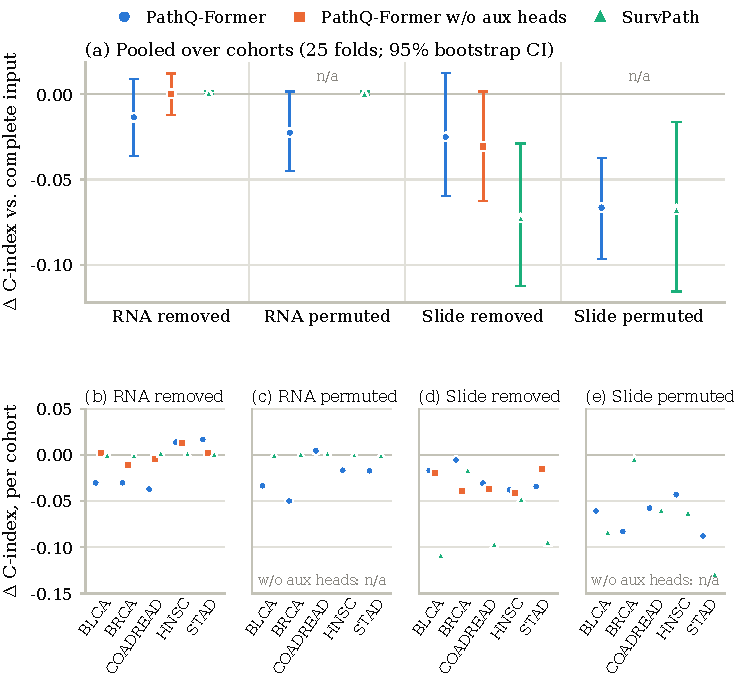
\includegraphics[width=0.9\linewidth]{figures/audit_deltas}
\caption{Change in \cindex{} of the same 20-epoch checkpoint when one test-time input is removed or permuted across validation patients, relative to its complete-input evaluation. SurvPath receives the training-mean gene vector or patch embedding for a removed input; \pq{} uses its learned null codes. (a) Pooled over the five cohorts: per (cohort, fold) the change is averaged over three seeds, then the mean and 95\% bootstrap confidence interval over the 25 folds are shown (10,000 resamples of folds). (b)--(e) The same quantity per cohort (mean over five folds). The variant without auxiliary heads was not evaluated under permutation (n/a).}
\label{fig:audit}
\end{figure}

The risk-score correlations say how the fused prediction is composed. For \pq{}, the Spearman $\rho$ between the fused risk and the same checkpoint's RNA-removed risk is 0.83 pooled over folds and seeds, against 0.45 with its slide-removed risk, and the two single-input risks correlate at 0.15 (Table~\ref{tab:corr}). The fused prediction therefore remains histology-led: the auxiliary heads make it respond to RNA, they do not make the two inputs symmetric. Its correlation with the other models' risks on the same fold and seed is 0.69 with the variant without auxiliary heads, 0.46 with SurvPath, 0.46 with ABMIL and 0.35 with the RNA MLP.

\subsection{Accuracy at equal budget}
\label{sec:accuracy}
Table~\ref{tab:acc} gives the \cindex{} of every method and Table~\ref{tab:tests} the seed-averaged paired tests. Pooled over 25 folds, \pq{} exceeds SurvPath by 0.036 (95\% CI $[-0.004, +0.071]$; $t$-test $p = 0.074$, Wilcoxon $p = 0.030$; 18 of 25 folds) and the variant without auxiliary heads by 0.037 ($[+0.009, +0.065]$; $p = 0.020$ and $0.020$; 17 of 25). Per cohort, BRCA is the only cohort with a raw $p < 0.05$ ($+0.086$, $t$-test $p = 0.017$), and it does not survive Holm correction over the five cohorts ($p = 0.084$); no DSS cohort survives correction (Table~\ref{tab:percohort}). Against the RNA-only MLP the margins are $+0.012$ and $+0.014$ ($p \ge 0.34$), and against the late-fusion ensemble $+0.011$ and $+0.009$ ($p \ge 0.28$; seeds 0--1); the MLP scores higher than \pq{} on BRCA and COADREAD and higher than the variant without auxiliary heads on BLCA and BRCA. No unimodal baseline differs from SurvPath pooled (ABMIL $+0.001$, SNN $-0.007$, MLP $+0.024$). The equal-budget result is therefore parity with the best unimodal baseline, not superiority. On overall survival (one seed) \pq{} leads SurvPath by 0.034 ($[+0.014, +0.054]$; $p = 0.003$ and $0.003$), and under a 10-epoch budget the variant without auxiliary heads leads by 0.028 ($p = 0.079$ and $0.063$); both are tabulated in Tables~\ref{tab:os} and~\ref{tab:e10}.

\begin{table}[t]
\caption{Disease-specific survival \cindex{} under the 20-epoch protocol: mean $\pm$ sample standard deviation over seeds of the five-fold mean (three seeds; late fusion two seeds; the BRCA cells of the single-modality \pq{}s two seeds). Pooled is the mean of the five cohort means. $^\dagger$Development cohort.}
\label{tab:acc}
\centering
\footnotesize
\setlength{\tabcolsep}{3pt}
\begin{tabular}{@{}llcccccc@{}}
\toprule
Method & Inputs & BLCA$^\dagger$ & BRCA & COADREAD & HNSC & STAD & Pooled \\
\midrule
\pq{} & WSI+RNA & \pmv{0.630}{0.010} & \pmv{0.622}{0.033} & \pmv{0.613}{0.023} & \pmv{0.582}{0.025} & \pmv{0.572}{0.022} & 0.604 \\
\pq{} w/o aux heads & WSI+RNA & \pmv{0.609}{0.016} & \pmv{0.611}{0.039} & \pmv{0.638}{0.031} & \pmv{0.575}{0.012} & \pmv{0.593}{0.015} & 0.605 \\
SurvPath & WSI+RNA & \pmv{0.594}{0.012} & \pmv{0.536}{0.026} & \pmv{0.570}{0.038} & \pmv{0.552}{0.019} & \pmv{0.587}{0.008} & 0.568 \\
Late fusion & WSI+RNA & \pmv{0.629}{0.018} & \pmv{0.606}{0.020} & \pmv{0.620}{0.069} & \pmv{0.571}{0.009} & \pmv{0.544}{0.006} & 0.594 \\
ABMIL & WSI & \pmv{0.566}{0.011} & \pmv{0.575}{0.004} & \pmv{0.587}{0.023} & \pmv{0.562}{0.028} & \pmv{0.553}{0.020} & 0.569 \\
Slide-only \pq{} & WSI & \pmv{0.592}{0.003} & \pmv{0.615}{0.027} & \pmv{0.574}{0.024} & \pmv{0.585}{0.003} & \pmv{0.582}{0.019} & 0.590 \\
SNN & RNA & \pmv{0.590}{0.009} & \pmv{0.558}{0.013} & \pmv{0.572}{0.028} & \pmv{0.535}{0.006} & \pmv{0.549}{0.009} & 0.561 \\
RNA MLP & RNA & \pmv{0.611}{0.012} & \pmv{0.627}{0.013} & \pmv{0.633}{0.016} & \pmv{0.555}{0.012} & \pmv{0.532}{0.009} & 0.592 \\
RNA-only \pq{} & RNA & \pmv{0.608}{0.020} & \pmv{0.559}{0.001} & \pmv{0.598}{0.035} & \pmv{0.554}{0.013} & \pmv{0.511}{0.005} & 0.566 \\
\bottomrule
\end{tabular}
\end{table}

\begin{table}[t]
\caption{Seed-averaged paired tests over the 25 pooled (cohort, fold) units: mean difference in \cindex{} (first minus second method), 95\% percentile-bootstrap CI (10,000 resamples of folds), paired $t$-test and exact Wilcoxon $p$-values, and folds won. Seeds are averaged per fold before pairing (three seeds for DSS; seeds 0--1 against late fusion; one seed for OS).}
\label{tab:tests}
\centering
\small
\setlength{\tabcolsep}{4pt}
\begin{tabular}{@{}llrlccc@{}}
\toprule
Comparison & Setting & $\Delta$ & 95\% CI & $t$ $p$ & W $p$ & Wins \\
\midrule
\pq{} vs SurvPath & DSS & $+0.036$ & $[-0.004, +0.071]$ & 0.074 & 0.030 & 18/25 \\
\pq{} w/o aux heads vs SurvPath & DSS & $+0.037$ & $[+0.009, +0.065]$ & 0.020 & 0.020 & 17/25 \\
ABMIL vs SurvPath & DSS & $+0.001$ & $[-0.024, +0.026]$ & 0.95 & 0.85 & 14/25 \\
SNN vs SurvPath & DSS & $-0.007$ & $[-0.060, +0.045]$ & 0.80 & 0.73 & 10/25 \\
RNA MLP vs SurvPath & DSS & $+0.024$ & $[-0.027, +0.077]$ & 0.38 & 0.41 & 15/25 \\
\pq{} vs RNA MLP & DSS & $+0.012$ & $[-0.022, +0.044]$ & 0.47 & 0.34 & 14/25 \\
\pq{} w/o aux heads vs RNA MLP & DSS & $+0.014$ & $[-0.023, +0.049]$ & 0.47 & 0.37 & 16/25 \\
\pq{} vs late fusion & DSS, seeds 0--1 & $+0.011$ & $[-0.013, +0.034]$ & 0.39 & 0.28 & 14/25 \\
\pq{} w/o aux heads vs late fusion & DSS, seeds 0--1 & $+0.009$ & $[-0.020, +0.036]$ & 0.54 & 0.52 & 14/25 \\
\pq{} vs SurvPath & OS, seed 0 & $+0.034$ & $[+0.014, +0.054]$ & 0.003 & 0.003 & 19/25 \\
\pq{} w/o aux heads vs SurvPath & DSS, 10 epochs & $+0.028$ & $[-0.001, +0.057]$ & 0.079 & 0.063 & 18/25 \\
\bottomrule
\end{tabular}
\end{table}


\subsection{Missing inputs at test time}
\label{sec:missing}
Figure~\ref{fig:missing} shows the random-missingness sweep. With half of the validation patients missing one modality, the fused \cindex{} of \pq{} changes by at most 0.025 (BRCA, 0.622 to 0.597) and that of the variant without auxiliary heads by at most 0.018 (BRCA). For \pq{} every change is within one sample seed standard deviation of the complete-input score (Table~\ref{tab:acc}); for the variant without auxiliary heads the HNSC and STAD changes (0.013 and 0.017) exceed it by 0.001 and 0.002. A site with mixed availability can instead route slide-only patients to ABMIL and RNA-only patients to the RNA MLP, or average the slide-only and RNA-only models when both inputs exist; routing and late fusion are robust by construction, and the late-fusion ensemble matches the joint model (Table~\ref{tab:tests}). The one-checkpoint result is about coverage, not accuracy: with the RNA removed, the single \pq{} checkpoint scores 0.576--0.600 against 0.553--0.587 for ABMIL (higher on four cohorts, lower on COADREAD); with the slide removed it scores 0.538--0.617 against 0.532--0.633 for the RNA MLP, higher on BLCA and STAD and lower on BRCA, COADREAD and HNSC (by up to 0.050 on COADREAD; three-seed means throughout).

\begin{figure}[t]
\centering
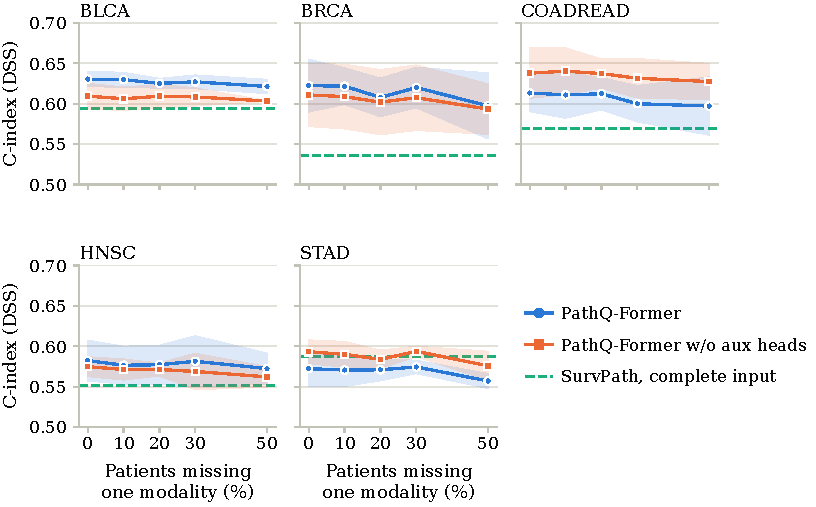
\includegraphics[width=0.85\linewidth]{figures/missing_rate_seeds}
\caption{\cindex{} of \pq{} and of its variant without auxiliary heads (20 epochs) when 0--50\% of validation patients are missing one modality at random (mean of five random draws per fold). Lines: mean over three seeds of the five-fold mean; bands: $\pm$1 sd over seeds. Dashed line: SurvPath with complete inputs (three-seed mean). With half the patients missing a modality the fused \cindex{} changes by at most 0.025 (BRCA).}
\label{fig:missing}
\end{figure}

\subsection{Where the robustness comes from}
\label{sec:where}
Evaluating the same checkpoints under mean imputation instead of the null code separates the two. For the variant without auxiliary heads, replacing the removed slide by the training-mean patch embedding instead of the null code turns a loss of 0.030 into a loss of 0.069 ($t$-test $p = 3 \times 10^{-4}$, Wilcoxon $p = 2.5 \times 10^{-4}$; one seed, 25 folds), the size of SurvPath's collapse; with the heads the loss is 0.035 under mean imputation ($p = 0.040$ and $0.045$; three seeds) against 0.025 with the null code (per-cohort values in Table~\ref{tab:impute}). The attribution is therefore: null codes and modality dropout remove the collapse without the slide, and the null code is what makes the checkpoint usable with the slide absent; the auxiliary heads are what makes the fused output respond to RNA; and the fused risk remains histology-led ($\rho$ 0.83 against 0.45). Fusion-block ablations on BLCA under the 10-epoch budget (modality dropout 0--0.5, 16--64 queries, fusion depth 1--3; one seed) move the fused \cindex{} within 0.595--0.638, inside the fold standard deviation of 0.07--0.13 (Table~\ref{tab:ablate}).

\subsection{Checkpoint selection on event-poor folds}
\label{sec:selection}
Every run stores its per-epoch validation history, so the effect of a selection rule can be replayed without training. Table~\ref{tab:selection} replays validation-loss early stopping with patience 5 on the 590 stored fold histories of the eight 20-epoch methods. The rule selects epoch 1 on median (mean 1.6; 93\% of folds epoch 1--3) and would have stopped after 6.6 of 20 epochs on average, with the patience limit reached in every fold. Pooled over the 25 seed-averaged folds, the early-stopped checkpoint scores below the final one by 0.090 for \pq{} without heads, 0.059 for \pq{}, 0.065 for the slide-only and 0.034 for the RNA-only \pq{}, 0.038 for SNN and 0.027 for the RNA MLP, and by nothing for ABMIL ($-0.001$) and SurvPath ($+0.000$). The histories show why: ABMIL and SurvPath reach their best validation \cindex{} at epoch 6.2 and 6.9 on average, SNN and the MLP at 7.2--7.3, and the \pq{} variants, which train with a warm-up epoch and a lower learning rate (Table~\ref{tab:training}) and are the late learners, at 9.3--10.0, so an epoch-1--2 checkpoint costs the late learners most. Under the replayed rule 23 of the 40 method $\times$ cohort cells have a mean \cindex{} within 0.45--0.55, against 5 under the final checkpoint (HNSC 8 of 8, STAD 7 of 8, BRCA 4 of 8). An earlier validation-loss run on these cohorts (120 folds) behaved the same way: median selected epoch 1 and 13 of 22 method $\times$ cohort cells within 0.45--0.55 (Appendix~\ref{app:runs}). Every replayed rule selects and scores on the same fold, so the measured deficit of early stopping is conservative. On cohorts with 5--45 events per validation fold, checkpoints should not be selected on the validation negative log-likelihood; a fixed budget with the final checkpoint, or at least the selected epochs and the events per fold, should be reported.

\begin{table}[t]
\caption{Replay of validation-loss early stopping (patience 5) on the stored 20-epoch histories (three seeds; the single-modality \pq{}s 70 instead of 75 fold histories). Final and early-stopped \cindex{}: pooled mean over (fold, seed) runs. $\Delta$: early-stopped minus final, paired over the 25 seed-averaged folds, with $t$-test and Wilcoxon $p$-values. Selected: mean epoch the rule selects; best val.: mean epoch of the highest validation \cindex{}. Selection and scoring use the same fold, so $\Delta$ is biased in favour of the rule. For the two single-modality \pq{}s this run-weighted mean differs by 0.001--0.002 from the Pooled column of Table~\ref{tab:acc}, which averages the five cohort means.}
\label{tab:selection}
\centering
\small
\begin{tabular}{@{}lccrccrr@{}}
\toprule
Method & Final & Early-stopped & $\Delta$ & $t$ $p$ & W $p$ & Selected & Best val. \\
\midrule
\pq{} & 0.604 & 0.546 & $-0.059$ & 0.016 & $8\times10^{-4}$ & 2.2 & 10.0 \\
\pq{} w/o aux heads & 0.605 & 0.516 & $-0.090$ & $3\times10^{-7}$ & $1\times10^{-6}$ & 1.8 & 9.9 \\
Slide-only \pq{} & 0.588 & 0.523 & $-0.065$ & 0.006 & 0.005 & 1.8 & 9.3 \\
RNA-only \pq{} & 0.567 & 0.532 & $-0.034$ & 0.062 & 0.080 & 1.4 & 9.7 \\
SurvPath (official) & 0.568 & 0.568 & $+0.000$ & 0.99 & 0.98 & 1.6 & 6.9 \\
ABMIL & 0.569 & 0.568 & $-0.001$ & 0.95 & 0.61 & 1.4 & 6.2 \\
SNN & 0.561 & 0.523 & $-0.038$ & 0.054 & 0.052 & 1.4 & 7.3 \\
RNA MLP & 0.592 & 0.565 & $-0.027$ & 0.078 & 0.075 & 1.2 & 7.2 \\
\bottomrule
\end{tabular}
\end{table}

\section{Discussion}
\label{sec:discussion}

\paragraph{A general lesson} Fusion of a strong and a weak modality can converge to ignoring the weak one with no accuracy signal: SurvPath's fused \cindex{} is as high as its slide-only behaviour permits, and nothing in the survival objective penalises leaving the genomic branch unused once the fusion block has found a low-loss route through the histology branch. This is the modality-competition effect that Gradient Blending~\citep{wang2020gradientblending} and OGM-GE~\citep{peng2022ogmge} describe for classification, and the same remedies apply: per-modality supervision supplies a direct gradient to the weak branch. The audit detects the failure without any training: removal and permutation across patients, with the risk-score correlation, show which input a ranking responds to, and they should accompany any multimodal \cindex{}. The audit also shows what unimodal supervision does and does not do here. It makes the fused output respond to RNA, but the fused risk still correlates at 0.83 with the same checkpoint's RNA-removed risk and at 0.45 with its slide-removed risk, and the RNA-permuted loss (0.023) is a third of the slide-permuted loss (0.067).

\paragraph{The RNA-only baseline} A two-layer MLP on bulk expression, run with repository defaults, matches both fusion variants pooled and scores higher than \pq{} on two of five cohorts. This baseline is cheap and seldom reported at equal budget; without it, an improvement attributed to fusion may be an improvement attributable to the genomic branch. Separating ``pathway tokens help'' from ``fusion helps'' would need an MLP that receives the same pathway tokens, which we have not run.

\paragraph{Limitations}
\begin{itemize}
\item \textbf{Baseline tuning and variant selection.} SurvPath was not re-tuned, and \pq{}'s hyper-parameters and the auxiliary-head variant were chosen as described under Scope of claims and in Appendix~\ref{app:training}. The accuracy comparison is favourable to \pq{} by an amount that cannot be bounded without tuning the baseline.
\item \textbf{Recipe on other architectures.} Null codes, modality dropout and auxiliary heads have not been applied to SurvPath, so how much of the robustness is specific to the query bottleneck is untested.
\item \textbf{Seeds and statistics.} Three seeds for the main comparison, two for late fusion, one for OS. Per-cohort tests have five folds; the fold-level standard deviation of the \cindex{} is 0.12--0.25 on COADREAD for the fusion models (0.05--0.25 over all methods), fold 3 of BLCA is weak for every method except the RNA-only \pq{}, and fold 0 of COADREAD, with five events, scores 0.85--0.92 for \pq{} across seeds. No per-cohort DSS difference survives correction; on OS (one seed) BLCA, the development cohort, does under the $t$-test only (Holm $p = 0.039$; Wilcoxon 0.312). The RNA-permuted loss of 0.023 that supports the auxiliary-head claim has $p = 0.075$ and $0.063$ over 25 folds.
\item \textbf{Data.} TCGA only, with frozen UNI2-h features whose pretraining corpus may include TCGA slides, which would make every WSI-based result optimistic; no external cohort; missingness simulated at random, so informative missingness is not covered; no clinical covariates (stage, grade, age), so whether any model adds to them is untested.
\end{itemize}

\section{Conclusion}
\label{sec:conclusion}
A fused histology--transcriptomics survival model can score well while its ranking ignores one input: the official SurvPath implementation, under an equal-budget protocol on five TCGA cohorts, does not respond to its RNA input and collapses without the slide. Removal and permutation audits with risk-score correlations detect this and should be reported with any multimodal \cindex{}. Training one fusion model with null codes and modality dropout removes the collapse, and auxiliary unimodal heads make the fused prediction respond to RNA; the resulting single checkpoint serves complete, slide-only and RNA-only patients; with both inputs it is not detectably different from an RNA-only MLP or a late-fusion ensemble, and with one input absent it stays within 0.05 of the dedicated unimodal baseline. Replaying checkpoint selection on the stored histories shows that validation-loss early stopping would have selected epoch 1--3 checkpoints and penalised the late-learning models on these event-poor folds, which argues for fixed budgets and for reporting selected epochs and events per fold.

\section*{Data and Code Availability}
TCGA data are public and de-identified. UNI2-h patch features~\citep{uni2h,uni2hfeatures} and the RNA-seq matrices, clinical metadata and splits released with SurvPath~\citep{jaume2024survpath} are available from their authors. The code (MIT licence), configuration files, archived per-run results (results, configuration, per-fold predictions and training histories for every run; inventory in Appendix~\ref{app:runs}) and the script that regenerates every table in Section~\ref{sec:results} and Appendix~\ref{app:tables} are included in the anonymized supplementary material. The 275 trained fold models (\pq{} and its variant without auxiliary heads at three seeds, SurvPath and the slide-only and RNA-only \pq{}s at seed 0, on the five cohorts, plus the two OS runs: 11 run configurations $\times$ five cohorts $\times$ five folds; 18 GB) will be released with the camera-ready version.
%% camera-ready: add public links here

\subsubsection*{Broader Impact Statement}
The model is a research prototype evaluated on public, de-identified TCGA data with simulated missingness. The model has not been validated on an external cohort, compared with clinical prognostic factors, or tested under informative missingness, and it must not be used to inform patient care. Performance across sex, race and age subgroups was not evaluated. The evaluation findings, that a fusion model can score well while its ranking is invariant to one input and that validation-loss checkpoint selection can leave methods near chance on event-poor cohorts, argue for reporting input-use audits, selection rules and events per fold in this literature.

\bibliography{references}
\bibliographystyle{tmlr}

\appendix

\section{Training Details and Selection History}
\label{app:training}

\paragraph{Query blocks} Each modality $m \in \{h, g\}$ has $K = 32$ learned queries $Q^m \in \mathbb{R}^{K \times d}$ with $d = 256$ and a stack of $L = 2$ pre-norm blocks,
\begin{align}
Q &\leftarrow Q + \mathrm{CA}\big(\mathrm{LN}(Q),\, U^m\big), \\
Q &\leftarrow Q + \mathrm{SA}\big(\mathrm{LN}(Q)\big), \\
Q &\leftarrow Q + \mathrm{FFN}\big(\mathrm{LN}(Q)\big),
\end{align}
where $U^m$ are the modality's input tokens (the LayerNormed patch embeddings, or the 275 pathway tokens produced by per-pathway two-layer MLPs of hidden width 128), $\mathrm{CA}$ is 8-head cross-attention with queries from $Q$ and keys and values from $U^m$, $\mathrm{SA}$ is self-attention among the queries and $\mathrm{FFN}$ is a two-layer feed-forward network. Cross-attention over $N$ input tokens costs $O(KNd)$ and attention among the queries $O(K^2 d)$; the block returns 32 vectors, so the fusion stage does not depend on $N$. The fused codes pass through two Transformer encoder layers ($d = 256$, 8 heads) and a learned-query attention pooling; a linear layer with a sigmoid produces the $T = 4$ hazards. Table~\ref{tab:training} gives the training configuration.

\begin{table}[htbp]
\caption{Training configuration of \pq{} and of the official SurvPath baseline.}
\label{tab:training}
\centering
\small
\begin{tabular}{@{}R{0.17\linewidth}R{0.42\linewidth}R{0.34\linewidth}@{}}
\toprule
Setting & \pq{} & SurvPath (official code) \\
\midrule
Epochs / selection & 20, final checkpoint & 20, final checkpoint \\
Optimizer & AdamW~\citep{loshchilov2019adamw}, lr $10^{-4}$, wd $10^{-4}$, 1 warm-up epoch, cosine decay & RAdam~\citep{liu2020variance}, lr $5 \times 10^{-4}$ (published), wd $10^{-4}$ \\
Batch & 1 patient, gradient accumulation 2, gradient clip 1.0 & 1 patient \\
Dropout & 0.25; modality dropout 0.15 & 0.1 \\
Patches & all patches of all slides & 4,096-patch subsample (published) \\
Loss & Eq.~\eqref{eq:nll}, censored term unweighted; auxiliary heads $\lambda = 0.5$ (full model) or $0$ & Eq.~\eqref{eq:nll}, censored term weighted 0.5 (published) \\
Sampling & uniform over training patients & weighted by (bin, censorship) (published) \\
Genes & min--max to $[-1, 1]$, fit on the training split & same \\
Parameters & 16.9\,M & 21.2\,M \\
\bottomrule
\end{tabular}
\end{table}

\paragraph{Selection history} The base hyper-parameters of \pq{} (learning-rate schedule, dropout, modality-dropout rate, number of queries, fusion depth) were chosen on BLCA under the 10-epoch budget from the single-seed ablation runs in Table~\ref{tab:ablate}; none of those settings is distinguishable from the others at one seed, and the chosen values are defaults rather than optima. The budget was raised from 10 to 20 epochs after inspecting the pooled validation curves of \pq{} and SurvPath under the 10-epoch budget; the 20-epoch curves (Figure~\ref{fig:epochs}) show SurvPath flat from about epoch 7 and both \pq{} variants rising until about epoch 13--18. The learning rate and gradient-accumulation setting of \pq{} were changed at the same time as the budget, so the 10- and 20-epoch results are not a pure budget comparison; a single-seed check at lr $2 \times 10^{-4}$ on BLCA did not improve on the default (0.615 vs 0.630). The auxiliary-head variant and $\lambda = 0.5$ were adopted after the 20-epoch results of the variant without auxiliary heads on all five cohorts had been seen; the two variants are therefore reported as co-primary throughout, and no per-cohort result on BLCA is treated as confirmatory. Best-epoch validation scores were logged in every run and are used only in the selection replay of Section~\ref{sec:selection}.

\begin{figure}[htbp]
\centering
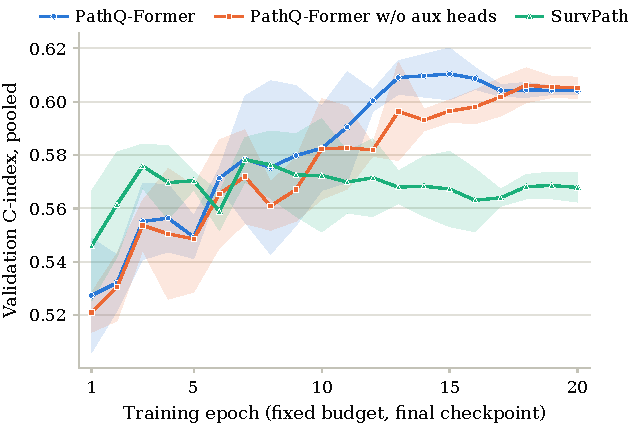
\includegraphics[width=0.5\linewidth]{figures/epoch_curves_pooled}
\caption{Validation \cindex{} per training epoch under the 20-epoch budget, pooled over all cohorts and folds; mean over three seeds with a $\pm$1 sd band over seeds, for \pq{}, its variant without auxiliary heads, and SurvPath. All results in the paper use the final epoch; the curves were inspected only to set the budget.}
\label{fig:epochs}
\end{figure}

\FloatBarrier
\section{Full Tables}
\label{app:tables}

\begin{table}[htbp]
\caption{Per-cohort seed-averaged paired differences in \cindex{} against SurvPath (five folds per cohort; three seeds for DSS, one seed for OS). Raw and Holm-adjusted $p$-values (over the five cohorts, $t$ and Wilcoxon adjusted separately) are computed from unrounded values. $^\dagger$Development cohort.}
\label{tab:percohort}
\centering
\small
\begin{tabular}{@{}lccccc@{}}
\toprule
 & BLCA$^\dagger$ & BRCA & COADREAD & HNSC & STAD \\
\midrule
\multicolumn{6}{@{}l}{\emph{\pq{} vs SurvPath (DSS, three seeds)}} \\
$\Delta$ & $+0.036$ & $+0.086$ & $+0.044$ & $+0.031$ & $-0.015$ \\
$t$ $p$ (Holm) & 0.175 (0.700) & 0.017 (0.084) & 0.583 (1.000) & 0.544 (1.000) & 0.719 (1.000) \\
W $p$ (Holm) & 0.312 (1.000) & 0.062 (0.312) & 0.625 (1.000) & 0.625 (1.000) & 0.625 (1.000) \\
wins & 3/5 & 5/5 & 4/5 & 4/5 & 2/5 \\
\midrule
\multicolumn{6}{@{}l}{\emph{\pq{} w/o aux heads vs SurvPath (DSS, three seeds)}} \\
$\Delta$ & $+0.015$ & $+0.075$ & $+0.068$ & $+0.023$ & $+0.006$ \\
$t$ $p$ (Holm) & 0.518 (1.000) & 0.073 (0.367) & 0.202 (0.807) & 0.580 (1.000) & 0.847 (1.000) \\
W $p$ (Holm) & 0.625 (1.000) & 0.125 (0.625) & 0.188 (0.750) & 0.625 (1.000) & 0.812 (1.000) \\
wins & 3/5 & 4/5 & 4/5 & 4/5 & 2/5 \\
\midrule
\multicolumn{6}{@{}l}{\emph{\pq{} vs SurvPath (OS, seed 0)}} \\
$\Delta$ & $+0.043$ & $+0.073$ & $-0.015$ & $+0.025$ & $+0.044$ \\
$t$ $p$ (Holm) & 0.008 (0.039) & 0.015 (0.058) & 0.578 (0.578) & 0.046 (0.138) & 0.230 (0.460) \\
W $p$ (Holm) & 0.062 (0.312) & 0.062 (0.312) & 0.625 (0.625) & 0.125 (0.375) & 0.312 (0.625) \\
wins & 5/5 & 5/5 & 2/5 & 4/5 & 3/5 \\
\bottomrule
\end{tabular}
\end{table}

\begin{table}[htbp]
\caption{Overall survival (20 epochs, seed 0): five-fold mean \cindex{} $\pm$ standard deviation over the five folds, and the \pq{} checkpoint evaluated with one input removed (null codes). Pooled: mean over the five cohorts. $^\dagger$Development cohort.}
\label{tab:os}
\centering
\small
\begin{tabular}{@{}lccccc@{}}
\toprule
 & & & & \multicolumn{2}{c}{\pq{}, one input removed} \\
\cmidrule(lr){5-6}
Cohort & \pq{} & SurvPath & $\Delta$ & RNA removed & Slide removed \\
\midrule
BLCA$^\dagger$ & \pmv{0.595}{0.053} & \pmv{0.552}{0.056} & $+0.043$ & 0.576 & 0.592 \\
BRCA & \pmv{0.596}{0.043} & \pmv{0.523}{0.052} & $+0.073$ & 0.531 & 0.556 \\
COADREAD & \pmv{0.581}{0.132} & \pmv{0.596}{0.153} & $-0.015$ & 0.586 & 0.562 \\
HNSC & \pmv{0.536}{0.036} & \pmv{0.510}{0.029} & $+0.025$ & 0.535 & 0.550 \\
STAD & \pmv{0.603}{0.070} & \pmv{0.559}{0.045} & $+0.044$ & 0.574 & 0.582 \\
\midrule
Pooled (25 folds) & 0.582 & 0.548 & $+0.034$ & & \\
\bottomrule
\end{tabular}
\end{table}

\begin{table}[htbp]
\caption{10-epoch budget (DSS, three seeds): \cindex{} mean $\pm$ sample standard deviation over seeds of the five-fold mean for \pq{} without auxiliary heads and SurvPath, with the seed-averaged paired difference over the five folds ($t$-test and Wilcoxon $p$-values). Pooled: 25 folds, 18 of 25 won. $^\dagger$Development cohort.}
\label{tab:e10}
\centering
\small
\begin{tabular}{@{}lccccc@{}}
\toprule
Cohort & \pq{} w/o aux heads & SurvPath & $\Delta$ & $t$ $p$ & W $p$ \\
\midrule
BLCA$^\dagger$ & \pmv{0.618}{0.014} & \pmv{0.589}{0.004} & $+0.029$ & 0.272 & 0.312 \\
BRCA & \pmv{0.600}{0.031} & \pmv{0.536}{0.015} & $+0.064$ & 0.142 & 0.188 \\
COADREAD & \pmv{0.646}{0.046} & \pmv{0.551}{0.022} & $+0.094$ & 0.015 & 0.062 \\
HNSC & \pmv{0.556}{0.007} & \pmv{0.568}{0.035} & $-0.013$ & 0.595 & 1.000 \\
STAD & \pmv{0.574}{0.025} & \pmv{0.607}{0.012} & $-0.033$ & 0.471 & 0.625 \\
\midrule
Pooled & 0.599 & 0.570 & $+0.028$ & 0.079 & 0.063 \\
\bottomrule
\end{tabular}
\end{table}

Table~\ref{tab:secondary} reports the secondary metrics. Uno's \cindex{} tracks Harrell's: \pq{} leads SurvPath by 0.039 ($[-0.016, +0.086]$; Wilcoxon $p = 0.042$) and the variant without auxiliary heads by 0.046 ($[+0.004, +0.087]$; $p = 0.045$ and $0.042$). Each of the four other methods in Table~\ref{tab:secondary} beats SurvPath on the integrated Brier score by about 0.07 (Wilcoxon $p < 10^{-4}$): SurvPath's hazards are poorly calibrated under this protocol (its published loss weights the censored term by 0.5), so the IBS is not a fair accuracy comparison and is reported for completeness only.

\begin{table}[htbp]
\caption{Secondary metrics under the 20-epoch DSS protocol: mean $\pm$ sample standard deviation over three seeds of the five-fold mean. Uno's IPCW \cindex{} is truncated at the 75th percentile of training event times; the integrated Brier score (IBS, lower is better) is evaluated on the interior quartile grid and is undefined on BRCA fold 4 for every method (cells marked * average four folds; the fold is dropped from the paired units, $n = 24$). $\Delta$ vs SurvPath: seed-averaged paired difference over the pooled folds with 95\% bootstrap CI, $t$-test and Wilcoxon $p$-values.}
\label{tab:secondary}
\centering
\footnotesize
\setlength{\tabcolsep}{3pt}
\begin{tabular}{@{}lccccc@{}}
\toprule
 & \pq{} & \begin{tabular}[c]{@{}c@{}}\pq{}\\ w/o aux heads\end{tabular} & ABMIL & RNA MLP & SurvPath \\
\midrule
\multicolumn{6}{@{}l}{\emph{Uno's IPCW \cindex{}}} \\
BLCA & \pmv{0.630}{0.009} & \pmv{0.612}{0.019} & \pmv{0.560}{0.014} & \pmv{0.605}{0.013} & \pmv{0.597}{0.010} \\
BRCA & \pmv{0.636}{0.012} & \pmv{0.648}{0.038} & \pmv{0.599}{0.012} & \pmv{0.598}{0.012} & \pmv{0.525}{0.049} \\
COADREAD & \pmv{0.616}{0.032} & \pmv{0.644}{0.009} & \pmv{0.629}{0.015} & \pmv{0.646}{0.025} & \pmv{0.592}{0.020} \\
HNSC & \pmv{0.589}{0.034} & \pmv{0.587}{0.012} & \pmv{0.563}{0.031} & \pmv{0.563}{0.013} & \pmv{0.556}{0.027} \\
STAD & \pmv{0.586}{0.019} & \pmv{0.601}{0.014} & \pmv{0.562}{0.029} & \pmv{0.550}{0.010} & \pmv{0.591}{0.011} \\
$\Delta$ vs SurvPath, $n = 25$ & $+0.039$ & $+0.046$ & $+0.010$ & $+0.020$ & \\
\quad 95\% CI & $[-0.016, +0.086]$ & $[+0.004, +0.087]$ & $[-0.019, +0.042]$ & $[-0.031, +0.070]$ & \\
\quad $t$ $p$ / W $p$ & 0.153 / 0.042 & 0.045 / 0.042 & 0.526 / 0.751 & 0.455 / 0.474 & \\
\midrule
\multicolumn{6}{@{}l}{\emph{Integrated Brier score}} \\
BLCA & \pmv{0.205}{0.008} & \pmv{0.210}{0.004} & \pmv{0.202}{0.007} & \pmv{0.191}{0.002} & \pmv{0.268}{0.031} \\
BRCA* & \pmv{0.073}{0.000} & \pmv{0.082}{0.004} & \pmv{0.077}{0.002} & \pmv{0.075}{0.002} & \pmv{0.131}{0.005} \\
COADREAD & \pmv{0.077}{0.006} & \pmv{0.081}{0.003} & \pmv{0.097}{0.001} & \pmv{0.082}{0.002} & \pmv{0.110}{0.009} \\
HNSC & \pmv{0.221}{0.019} & \pmv{0.215}{0.011} & \pmv{0.205}{0.010} & \pmv{0.200}{0.005} & \pmv{0.341}{0.087} \\
STAD & \pmv{0.201}{0.006} & \pmv{0.189}{0.009} & \pmv{0.208}{0.013} & \pmv{0.204}{0.001} & \pmv{0.276}{0.043} \\
$\Delta$ vs SurvPath, $n = 24$ & $-0.070$ & $-0.071$ & $-0.068$ & $-0.075$ & \\
\quad 95\% CI & $[-0.100, -0.044]$ & $[-0.101, -0.043]$ & $[-0.100, -0.039]$ & $[-0.108, -0.044]$ & \\
\quad $t$ $p$ / W $p$ & $<$0.001 / $<$0.001 & $<$0.001 / $<$0.001 & $<$0.001 / $<$0.001 & $<$0.001 / $<$0.001 & \\
\bottomrule
\end{tabular}
\end{table}

\begin{table}[htbp]
\caption{Risk-score correlations of \pq{} (20 epochs): Spearman $\rho$, mean $\pm$ standard deviation over the 15 (fold, seed) pairs, between the fused risk and the same checkpoint's single-input risks (left) and the other methods' risks on the same fold and seed (right). Pooled: mean over the 75 pairs.}
\label{tab:corr}
\centering
\footnotesize
\begin{tabular}{@{}lcccccc@{}}
\toprule
Fused risk of \pq{} vs & BLCA & BRCA & COADREAD & HNSC & STAD & Pooled \\
\midrule
own slide-removed risk & \pmv{0.42}{0.13} & \pmv{0.36}{0.12} & \pmv{0.53}{0.20} & \pmv{0.47}{0.08} & \pmv{0.45}{0.20} & 0.45 \\
own RNA-removed risk & \pmv{0.90}{0.08} & \pmv{0.85}{0.08} & \pmv{0.73}{0.14} & \pmv{0.84}{0.09} & \pmv{0.82}{0.16} & 0.83 \\
\quad (slide-removed vs RNA-removed) & \pmv{0.22}{0.07} & \pmv{0.09}{0.08} & \pmv{0.16}{0.19} & \pmv{0.15}{0.10} & \pmv{0.13}{0.23} & 0.15 \\
\midrule
\pq{} w/o aux heads & \pmv{0.79}{0.06} & \pmv{0.62}{0.14} & \pmv{0.66}{0.09} & \pmv{0.71}{0.10} & \pmv{0.69}{0.13} & 0.69 \\
SurvPath & \pmv{0.63}{0.08} & \pmv{0.38}{0.17} & \pmv{0.38}{0.09} & \pmv{0.45}{0.24} & \pmv{0.48}{0.12} & 0.46 \\
ABMIL & \pmv{0.46}{0.14} & \pmv{0.51}{0.17} & \pmv{0.38}{0.11} & \pmv{0.44}{0.13} & \pmv{0.48}{0.11} & 0.46 \\
RNA MLP & \pmv{0.42}{0.09} & \pmv{0.26}{0.08} & \pmv{0.37}{0.20} & \pmv{0.29}{0.06} & \pmv{0.41}{0.19} & 0.35 \\
SNN & \pmv{0.38}{0.11} & \pmv{0.23}{0.09} & \pmv{0.36}{0.16} & \pmv{0.29}{0.07} & \pmv{0.43}{0.21} & 0.34 \\
\bottomrule
\end{tabular}
\end{table}

\begin{table}[htbp]
\caption{Null code against mean imputation on the same \pq{} checkpoints (20 epochs): \cindex{} with one input replaced by the training-mean patch embedding or gene vector, mean $\pm$ sample standard deviation over three seeds of the five-fold mean (as in Table~\ref{tab:acc}; one seed, hence no sd, for the variant without auxiliary heads), and the pooled difference from the complete-input score over the 25 seed-averaged folds with $t$-test and Wilcoxon $p$-values. The null-code rows are those of Table~\ref{tab:audit}.}
\label{tab:impute}
\centering
\footnotesize
\setlength{\tabcolsep}{3pt}
\begin{tabular}{@{}lcccccrcc@{}}
\toprule
Condition & BLCA & BRCA & COADREAD & HNSC & STAD & $\Delta$ & $t$ $p$ & W $p$ \\
\midrule
\multicolumn{9}{@{}l}{\emph{\pq{}, mean imputation (three seeds)}} \\
RNA removed & \pmv{0.597}{0.003} & \pmv{0.607}{0.035} & \pmv{0.602}{0.012} & \pmv{0.589}{0.014} & \pmv{0.581}{0.018} & $-0.009$ & 0.29 & 0.49 \\
Slide removed & \pmv{0.595}{0.027} & \pmv{0.591}{0.060} & \pmv{0.580}{0.016} & \pmv{0.558}{0.024} & \pmv{0.521}{0.037} & $-0.035$ & 0.040 & 0.045 \\
\midrule
\multicolumn{9}{@{}l}{\emph{\pq{} w/o aux heads, mean imputation (one seed)}} \\
RNA removed & 0.627 & 0.545 & 0.631 & 0.580 & 0.594 & $-0.010$ & 0.50 & 0.83 \\
Slide removed & 0.524 & 0.499 & 0.600 & 0.535 & 0.524 & $-0.069$ & $3\times10^{-4}$ & $2.5\times10^{-4}$ \\
\bottomrule
\end{tabular}
\end{table}

\begin{table}[htbp]
\caption{Fusion-block ablations on BLCA under the 10-epoch budget (\pq{} without auxiliary heads, seed 0): five-fold mean \cindex{} $\pm$ standard deviation over the five folds with both inputs, and the same checkpoint with the RNA or the slide removed (null codes). The settings are not distinguishable at one seed.}
\label{tab:ablate}
\centering
\small
\begin{tabular}{@{}lccc@{}}
\toprule
Variant & Both inputs & RNA removed & Slide removed \\
\midrule
Base ($K = 32$, fusion depth 2, modality dropout 0.15) & \pmv{0.609}{0.069} & 0.602 & 0.630 \\
Modality dropout 0 & \pmv{0.634}{0.075} & 0.609 & 0.598 \\
Modality dropout 0.3 & \pmv{0.616}{0.068} & 0.624 & 0.648 \\
Modality dropout 0.5 & \pmv{0.635}{0.108} & 0.587 & 0.626 \\
$K = 16$ queries & \pmv{0.638}{0.070} & 0.615 & 0.615 \\
$K = 64$ queries & \pmv{0.634}{0.127} & 0.619 & 0.624 \\
Fusion depth 1 & \pmv{0.598}{0.124} & 0.584 & 0.611 \\
Fusion depth 3 & \pmv{0.595}{0.088} & 0.585 & 0.610 \\
\bottomrule
\end{tabular}
\end{table}

\FloatBarrier
\section{Efficiency}
\label{app:efficiency}
Table~\ref{tab:efficiency} reports parameters, latency and peak GPU memory per patient on the first 40 patients of the BLCA fold-0 validation set (medians, one RTX PRO 4000). At 4,096--6,214 patches the two models have equal forward latency; \pq{}'s training step takes 104\,ms against 176\,ms for SurvPath, and its peak memory on full slides is 1.17\,GiB against 1.74\,GiB. The claim is limited to these slide sizes on this GPU; neither implementation was profiled, and training throughput in practice was bound by reading features from storage.

\begin{table}[htbp]
\caption{Compute per patient on the first 40 patients of the BLCA fold-0 validation set (medians, one RTX PRO 4000). ``All patches'' is the median patient (6,214 patches).}
\label{tab:efficiency}
\centering
\small
\begin{tabular}{@{}lrrrrr@{}}
\toprule
Model & Params (M) & Patches & Fwd (ms) & Fwd+bwd (ms) & Peak mem.\ (GiB) \\
\midrule
\pq{}, all patches & 16.9 & 6,214 & 35.0 & 104.2 & 1.17 \\
\pq{}, 4,096 patches & 16.9 & 4,096 & 34.7 & 104.1 & 0.17 \\
SurvPath, 4,096 patches (as trained) & 21.2 & 4,096 & 35.7 & 175.6 & 0.20 \\
SurvPath, all patches & 21.2 & 6,214 & 36.0 & 176.0 & 1.74 \\
\bottomrule
\end{tabular}
\end{table}

\FloatBarrier
\section{Pathway Attention}
\label{app:pathways}
The genomic query block exposes cross-attention from each query over the 275 pathway tokens. Figure~\ref{fig:pathways} shows, per cohort, the eight tokens with the highest mean attention relative to uniform ($1/275$), averaged over validation patients and the five folds (seed 0). The top entries are 3.9 to 18.3 times the uniform weight, but the standard deviation over folds exceeds the mean for most of them (BLCA: apical junction, $6.7 \pm 7.9$; BRCA: glycolysis, $18.3 \pm 14.2$), so the ranking is descriptive only; attention weights are not a measure of feature importance~\citep{jain2019attention}.

\begin{figure}[htbp]
\centering
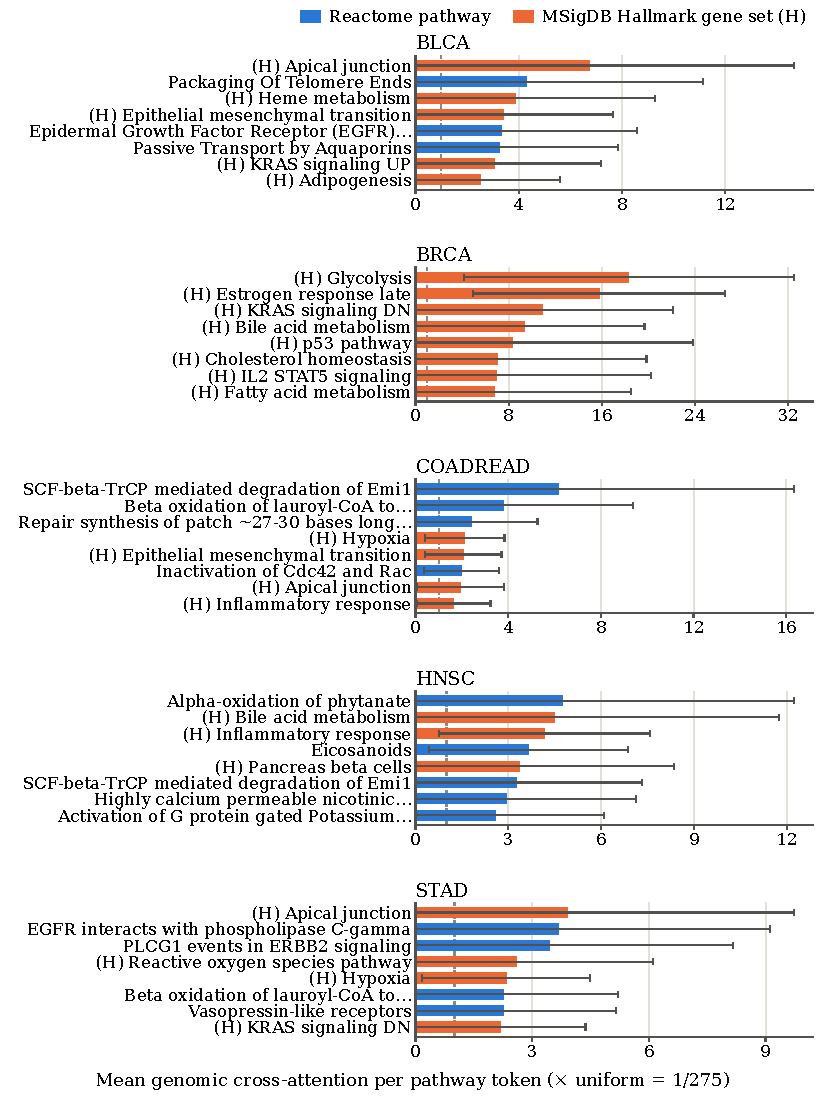
\includegraphics[width=\linewidth,height=0.88\textheight,keepaspectratio]{figures/pathway_importance_v2}
\caption{Pathway tokens with the highest mean genomic-query attention per cohort (\pq{}, 20 epochs, seed 0), as a multiple of uniform attention over the 275 tokens (dashed line), averaged over validation patients and the five folds. Blue: Reactome pathways; orange, marked (H): MSigDB Hallmark gene sets. Error bars span the mean $\pm$ the standard deviation over the five folds, clipped at zero. Names longer than 45 characters are shortened with an ellipsis.}
\label{fig:pathways}
\end{figure}

\section{Kaplan--Meier Curves}
\label{app:km}
Figure~\ref{fig:km} shows disease-specific survival of the high- and low-risk halves of the pooled out-of-fold predictions (20 epochs, seed 0). The log-rank $p$-values between the halves are, for \pq{}, 0.008 (BLCA), 0.054 (BRCA), 0.38 (COADREAD), 0.003 (HNSC) and 0.076 (STAD), and for SurvPath 0.014, 0.035, 0.96, 0.86 and $3 \times 10^{-5}$. The pooled curves combine five fold models at one seed and are descriptive.

\begin{figure}[htbp]
\centering
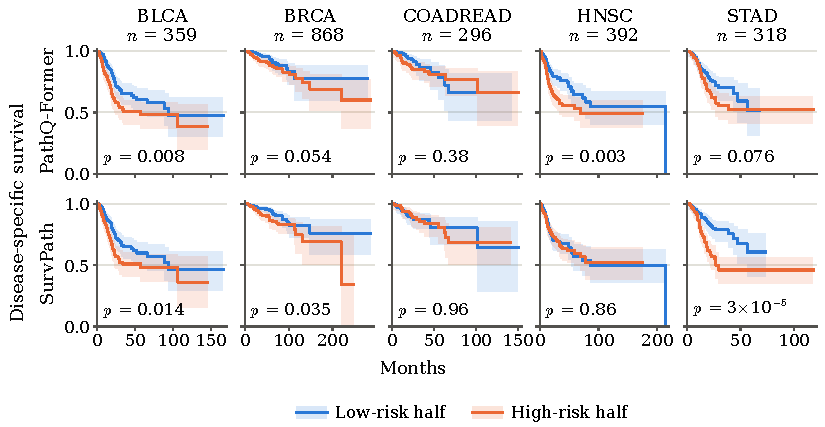
\includegraphics[width=\linewidth]{figures/km_grid}
\caption{Kaplan--Meier curves of disease-specific survival for the high- and low-risk halves of the pooled out-of-fold validation predictions (20 epochs, seed 0). Top row: \pq{}; bottom row: SurvPath; columns: the five cohorts with the pooled number of patients. Within each fold, patients are split at the median predicted risk of that fold's validation set, and the five folds are then pooled, so every patient appears once. Shaded bands: 95\% confidence intervals; $p$: two-sample log-rank test between the pooled halves.}
\label{fig:km}
\end{figure}

\section{Evaluation Pitfalls in Survival MIL Pipelines}
\label{app:pitfalls}
The following choices each produce plausible-looking \cindex{} values and are easy to make in a survival MIL pipeline; our pipeline avoids them as stated.
\begin{enumerate}
\item \textbf{Concordance on discrete bins.} Computing the \cindex{} on the four hazard bins ties a large fraction of the pairs; Harrell's \cindex{} is computed on continuous follow-up time.
\item \textbf{Bin edges fit on the validation fold.} Fitting the quartile edges separately on validation patients puts their labels on a different scale and leaks the validation label distribution; edges are fit on uncensored training patients and reused.
\item \textbf{Slide-level samples.} Counting each slide as a sample weights multi-slide patients several times and inflates the apparent cohort size; one sample per patient, with all slides concatenated.
\item \textbf{Unscaled gene inputs.} Feeding log-expression values on an arbitrary scale to per-pathway MLPs; genes are min--max scaled with training-split statistics.
\item \textbf{Selection on the reported fold.} Selecting a checkpoint on the validation fold that is also the reported fold biases every selection rule upward (Section~\ref{sec:selection}); a fixed budget with the final checkpoint and several seeds avoids it.
\item \textbf{Non-standard risk and dropout semantics.} Using $1 - S(T)$ as the risk score, or applying modality dropout per batch rather than per sample; risk is $-\sum_t S(t)$ and dropout is per sample.
\item \textbf{Extreme times in the Brier-score grid.} A grid that includes the minimum and maximum validation times evaluates on time points at which a single patient is at risk; the interior quartile edges are used.
\item \textbf{Untruncated IPCW weights.} Uno's \cindex{} diverges when the censoring survival function approaches zero at late times; it is truncated at the 75th percentile of training event times.
\end{enumerate}

\FloatBarrier
\section{Run Inventory and Compute}
\label{app:runs}
The archive holds 204 cohort-level runs, each of five folds: 34 under the earlier validation-loss protocol and the single-seed 10-epoch runs of \pq{} and SurvPath on five cohorts; 31 BLCA fusion-block ablations, late fusion and 10-epoch seeds 1--2 of \pq{} and SurvPath; 128 under the 20-epoch DSS protocol (the nine methods of Table~\ref{tab:methods} on five cohorts with the seeds listed there); 10 under the OS endpoint (\pq{} and SurvPath on five cohorts); and one 20-epoch learning-rate check on BLCA (Appendix~\ref{app:training}). The validation-loss protocol (patience 5, minimum 6 epochs, 120 folds) selected epoch 1 on median (82\% of folds epoch 1--3), trained 7.2 epochs on average, and reported a mean \cindex{} of 0.542 against 0.642 at the best epoch, with 13 of 22 method $\times$ cohort cells within 0.45--0.55; SurvPath on STAD (0.610) and SNN on BRCA (0.572) are among the exceptions. Every trained run stores its results, configuration, per-fold predictions and per-epoch training histories (the late-fusion runs store results and per-fold predictions only); the tables of Section~\ref{sec:results} and Appendix~\ref{app:tables} are regenerated from these files by one script. GPU runs were executed on rented RTX PRO 4000/4500 and RTX 2000 Ada GPUs sharing a network volume; throughput was bound by feature I/O rather than by either model.

\end{document}
